A distribuição dos autovalores de uma matriz aleatória Gaussiana $N\times N$ é dada por:

\begin{equation}
	\rho(\mmany{x}{N}) = \frac{1}{\mathcal{Z}_{N,\beta}} e^{-\frac{1}{2} \sum_{i=1}^{N} x_i^2} \prod_{j<k} |x_j - x_k|^{\beta}
	\label{eq: dist geral gaussiana}
\end{equation}

onde a constante de normalização $\mathcal{Z}$ é dada por

\begin{equation}
		\mathcal{Z}_{N, \beta} = (2\pi)^{\frac{N}{2}} \prod_{j=1}^{N} \frac{\Gamma (1 + j \frac{\beta}{2})}{\Gamma (1 + \frac{\beta}{2})}
\end{equation}

$\beta$ é o index de Dyson e indica o ensemble que utilizamos. Mais importante é notar que existe na nossa distribuição um fator de repulsão e um fator de campo de mínimo de energia em $x=0$. De forma que mesmo centradas em $0$ as partículas mantém uma distância entre si pela repulsão 'Coulombiana'.

Se quisermos computar o histograma dos autovalores podemos tomar a marginal

\begin{equation}
	\rho(x) = \int \cdots \int \mcmany{dx}{N}{\cdot} \rho(x, x_2, \cdots, x_N)
\end{equation}

Ou seja, o perfil da função partição de uma nova partícula dada o posicionamento das outras. Para a Equação \ref{eq: dist geral gaussiana}, a densidade espectral $\mathbb{E}[n(x)]=\rho(x)$ é dada pelo limite

\begin{equation}
	\lim_{N \rightarrow \infty} \sqrt{\beta N} \rho(\sqrt{\beta N} x) = \rho_{sc}(x)
\end{equation}

Onde $\rho_{sc}(x) = \frac{1}{\pi} \sqrt{2 - x^2}$ compõe a famosa lei do semi-círculo de Wigner representada na Figura \ref{fig: lambdadist}. Os pontos $\pm \sqrt{2 \beta N}$ são as bordas espectrais. Um esquema útil para organização dos multiplos ensembles é a classificação de Layman. Denomina-se

\begin{enumerate}
	\item \textbf{Entradas Independentes}: Adicionada a necessidade de simetria, matrizes deste tipo são chamadas matrizes de Wigner.
	\item \textbf{Invariantes por rotação}: Quaisquer duas matrizes que são relacionadas por uma transformação $\matriz{H'} = \matriz{U} \matriz{H} \matriz{U}^{-1}$ ocorrerão com a mesma probabilidade.
\end{enumerate}

Só existe um tipo especial de matriz que se encontra na intersecção e são as classes Gaussianas.

Em geral no mundo das matrizes aleatórias três classes são muito importantes e serão atores centrais no nosso estudo. São as três classes associadas às matrizes que tem entradas gaussianas. Estas são: O Ensemble Gaussiano Ortogonal (GOE), O Ensemble Gaussiano Unitário (GUE) e o Ensemble Gaussiano Simplético (GSE). Em suma, eles tratam, em ordem, de matrizes com entradas gaussianas reais, complexas e quaterniônicas. Seus nomes estão relacionados com a matriz necessária para a transformação de diagonalização das matrizes. Unitária para o caso complexo, por exemplo. Seus autovalores possuem distribuições distintas (ao menos para a escala usada) e é ilustrada abaixo na Figura \eqref{fig: lambdadist}.

\begin{center}
	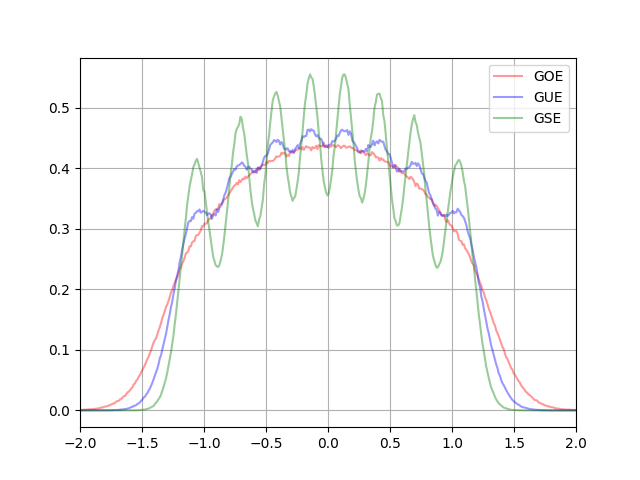
\includegraphics[width=0.8\linewidth]{FullGaussianDensityEscaled.png}
	\label{fig: lambdadist}
\end{center}

Mais desenvolvimento sobre a forma desta distribuição e as diferenças será feito posteriormente. Usaremos a referência \cite{Livan_2018} para a maior parte dos desenvolvimentos. Algum material interessante pode ser consultado em um livro de física em \cite{MEHTA1967v}.